\documentclass[conference]{IEEEtran}
\IEEEoverridecommandlockouts
\usepackage{cite}
\usepackage{amsmath,amssymb,amsfonts}
\usepackage{algorithmic}
\usepackage{graphicx}
\usepackage{textcomp}
\usepackage{xcolor}
\usepackage{booktabs}
\usepackage{float}
\usepackage{multirow}
\usepackage{siunitx}
\usepackage[hyphens]{url}

\def\BibTeX{{\rm B\kern-.05em{\sc i\kern-.025em b}\kern-.08em
    T\kern-.1667em\lower.7ex\hbox{E}\kern-.125emX}}

\graphicspath{{../results/plots/}}

\begin{document}

\title{Topological Risk Analysis and Criticality Mapping\\ in the npm Software Supply Chain}

\author{\IEEEauthorblockN{Yusuf Talha ARABACI}
\IEEEauthorblockA{\textit{Department of Software Engineering} \\
\textit{Karabuk University}\\
Karabuk, Turkey \\
yusuftalhaarabaci@hotmail.com}
}

\maketitle

\begin{abstract}
The Node Package Manager (npm) ecosystem, while essential for modern software development, forms a complex dependency network where localized failures can precipitate cascading effects across the supply chain. Conventional security analyses, which often inspect package source code for vulnerabilities, tend to overlook systemic risks embedded in the topological structure of the dependency graph. This paper introduces the Behavioral Risk Score (BRS), a content-independent, multi-metric model for identifying structurally critical packages. We constructed a dependency graph of 1,506 packages and 3,058 dependencies and analyzed its topological properties. The BRS model synthesizes weighted metrics—including betweenness centrality, degree centrality, and clustering coefficient—into a single score. Our analysis reveals that the network exhibits a scale-free topology, where risk is concentrated within a small number of nodes. The package `@babel/helper-plugin-utils` was identified as having the highest BRS, indicating its role as a structural linchpin. The results also demonstrate a distinction between a package's structural importance within our constructed graph and its broader ecosystem impact. This study proposes a topology-based methodology for prioritizing security resources, arguing that focusing on structurally critical nodes is a more efficient strategy for mitigating systemic risk.
\end{abstract}

\begin{IEEEkeywords}
Software supply chain security, npm, dependency network, topological analysis, risk scoring, network robustness.
\end{IEEEkeywords}

\section{Introduction}
Modern software engineering is heavily reliant on centralized package managers such as npm, which host vast repositories of reusable code libraries \cite{wyss2025npm}. This modularity accelerates development but also creates a fragile software supply chain where a single point of failure can propagate throughout the ecosystem \cite{duan2020measuring}. With millions of packages and complex inter-dependencies, the npm ecosystem presents a large attack surface \cite{wang2023threat}. Vulnerabilities can spread uncontrollably through the dependency graph \cite{liu2022demystifying, zerouali2022impact}, and disruptions in package maintenance further compound these systemic risks \cite{rahman2024update, cogo2020maintenance}.

The literature confirms that the npm network exhibits "small-world" characteristics, wherein a few key packages or maintainers have a disproportionate influence \cite{zimmermann2019smallworld, oldnall2017complex}. This topological structure makes the ecosystem vulnerable to a range of supply chain attacks, from typosquatting to the compromise of trusted, popular packages \cite{ohm2020backstabber}. Although various defense mechanisms based on machine learning, dynamic analysis, and metadata scanning have been proposed \cite{sejfia2022amalfi, zheng2024oscar, halder2024metadata}, the sheer scale of the ecosystem makes comprehensive code-level scanning of every package unfeasible.

Existing research often quantifies risk based on known vulnerabilities or package maintenance status. A gap exists, however, in approaches that quantify systemic risk arising from the network's topological architecture alone. This study addresses this gap by introducing a model that is independent of package content, focusing exclusively on structural dependencies. We propose the \textbf{Behavioral Risk Score (BRS)}, a composite metric that weights various centrality measures to identify and prioritize structurally critical packages. Our objective is to provide a quantitative framework for security resource allocation, enabling a more strategic defense against systemic supply chain threats.

\section{Methodology}
\subsection{Dataset and Network Construction}
A sampling strategy centered on systemic impact, rather than raw download counts, was adopted. Accordingly, the top 1,000 packages with the highest dependent counts were selected from the \texttt{ecosyste.ms} dataset to form the seed set. All dependencies of this seed set, up to a depth of seven, were included in the analysis. Following a data preprocessing step where circular references were removed, a directed graph of \textbf{1,506 nodes (packages)} and \textbf{3,058 edges (dependencies)} was constructed. The Python NetworkX library was used for all network modeling and analysis.

\subsection{The Behavioral Risk Score (BRS) Model}
The BRS is a composite score designed to provide a holistic view of a package's structural risk. It synthesizes multiple metrics to combine the network's topological structure with the package's prevalence in the ecosystem.

First, the following centrality metrics are calculated for each package:
\begin{itemize}
    \item \textbf{In-Degree:} The number of incoming dependencies. It is an indicator of a package's popularity and direct impact.
    \item \textbf{Out-Degree:} The number of outgoing dependencies. A high out-degree may indicate an increased attack surface.
    \item \textbf{Betweenness Centrality:} The frequency with which a package appears on the shortest paths between other packages, indicating its role as a "bridge" in the network.
    \item \textbf{Clustering Coefficient:} A measure of how connected a package's neighbors are to each other. A low value suggests a role as a bridge between distinct clusters.
\end{itemize}
In addition to these topological metrics, we include the total \textbf{Dependents Count} and \textbf{Download Count} from the wider ecosystem as proxies for global adoption.

Before inclusion in the BRS, each metric is normalized to a $[0,1]$ range using the Min-Max method:
\begin{equation}
x' = \frac{x - \min(x)}{\max(x) - \min(x)}
\end{equation}
where $x$ is the raw value of the metric and $x'$ is its normalized value.

The final BRS is calculated as a weighted sum of the normalized metrics:
$$
\begin{aligned}
\text{BRS} = & \ 0.40 \cdot \text{Betweenness}' + 0.20 \cdot \text{InDegree}' \\
& + 0.10 \cdot \text{OutDegree}' + 0.10 \cdot \text{Clustering}' \\
& + 0.10 \cdot \text{Dependents}' + 0.10 \cdot \text{Downloads}'
\end{aligned}
$$

The rationale for this weighting is as follows:
\begin{itemize}
    \item \textbf{Betweenness ($w=0.40$)}: The highest weight is assigned to "bridge" nodes that control information and risk flow. This is based on the hypothesis that a package's strategic position is more critical than its popularity in the propagation of cascading failures.
    \item \textbf{In-Degree ($w=0.20$)}: Represents the package's direct impact radius.
    \item \textbf{Other Metrics ($w=0.10$ each)}: Global metrics (Dependents, Downloads) and local structural metrics (Out-Degree, Clustering) are included to create a balanced, hybrid risk score.
\end{itemize}

\subsection{Robustness and Cascade Analysis}
To test the model's validity, targeted attack simulations were performed. The effects on the Largest Connected Component (LCC) size and overall network accessibility were analyzed by removing high-BRS packages. The predictive power of the model was further verified by a cascade analysis.

\section{Results and Discussion}

\subsection{Network Topology and Structural Characteristics}
The constructed dependency network exhibits a clustered topology (Figure \ref{fig:network}) and a scale-free structure. The degree distributions for both in-degree and out-degree show a heavy-tailed pattern (Figure \ref{fig:histograms}), which is characteristic of scale-free networks. This indicates that a small number of packages act as central hubs, while the majority of nodes have few connections. This structure suggests that systemic risk is not uniformly distributed but is concentrated within a subset of critical packages.

\begin{figure}[H]
\centering
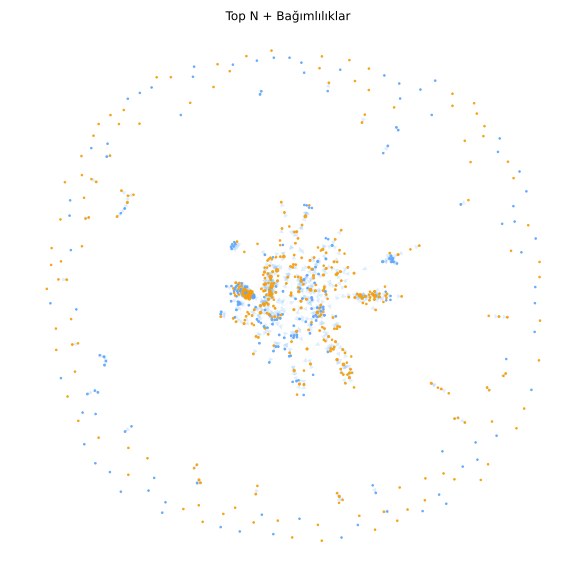
\includegraphics[width=\linewidth]{network_full_topN.png}
\caption{Visualization of the analyzed dependency network. Dense regions indicate distinct sub-clusters of packages.}
\label{fig:network}
\end{figure}

\begin{figure}[H]
\centering
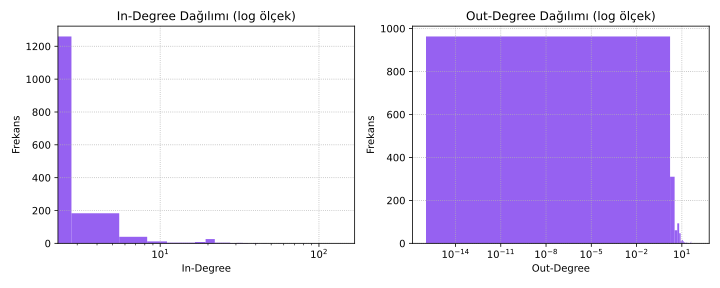
\includegraphics[width=\linewidth]{degree_histograms.png}
\caption{In-degree and out-degree histograms, showing a heavy-tailed distribution characteristic of a scale-free network.}
\label{fig:histograms}
\end{figure}

\subsection{Centrality Relationships}
An analysis of centrality measures reveals an asymmetric relationship between a package's popularity (in-degree) and its structural importance as a bridge (betweenness centrality), as shown in the correlation matrix in Figure \ref{fig:scatter}. The weak correlation suggests that some packages with low popularity may still be critical to the network's integrity by connecting otherwise disparate components. Consequently, security analyses that focus exclusively on popularity metrics such as download counts are likely to overlook these structural risks.

\begin{figure}[H]
\centering
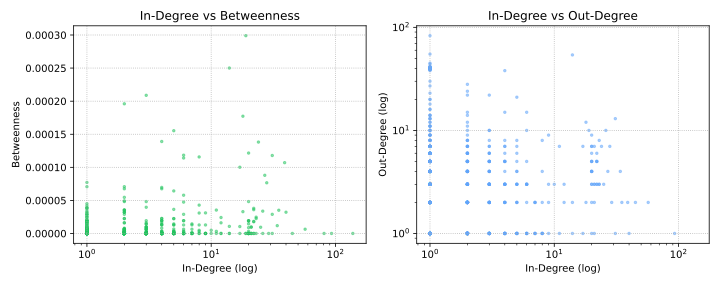
\includegraphics[width=\linewidth]{scatter_correlations.png}
\caption{Correlations between network centrality measures.}
\label{fig:scatter}
\end{figure}

\subsection{Analysis of Critical Nodes}
Tables \ref{tab:indegree}, \ref{tab:outdegree}, and \ref{tab:betweenness} list the top 10 packages for each respective centrality measure. Packages with a high in-degree, such as \texttt{@babel/helper-plugin-utils}, are widely used dependencies. Those with a high out-degree, such as \texttt{@babel/preset-env}, have a large number of dependencies themselves, which can indicate an increased attack surface. Packages with high betweenness centrality are critical for network integrity, acting as bridges. For example, \texttt{jest-circus} has a low in-degree of 1 but the highest betweenness score, demonstrating its importance as a structural bridge. In contrast, a package like \texttt{@babel/core} has both high popularity (in-degree) and a high betweenness score. These results show that no single metric is sufficient for a complete risk analysis and highlight the importance of identifying structurally critical bridge packages.

\begin{table}[H]
\centering
\caption{\textsc{Top 10 Packages by In-Degree Centrality}}
\label{tab:indegree}
\resizebox{\linewidth}{!}{%
\begin{tabular}{lrrrr}
\toprule
Package & In-Degree & Out-Degree & Betweenness & TopN? \\
\midrule
@babel/helper-plugin-utils & 110 & 0 & 0.000000 & True \\
call-bound & 41 & 2 & 0.000283 & False \\
postcss-value-parser & 39 & 0 & 0.000000 & True \\
call-bind & 36 & 4 & 0.000000 & False \\
@types/node & 34 & 1 & 0.000067 & False \\
debug & 34 & 1 & 0.000100 & True \\
es-errors & 33 & 0 & 0.000000 & False \\
@babel/types & 32 & 2 & 0.000236 & True \\
define-properties & 29 & 3 & 0.000000 & False \\
chalk & 28 & 0 & 0.000000 & False \\
\bottomrule
\end{tabular}%
}
\end{table}

\begin{table}[H]
\centering
\caption{\textsc{Top 10 Packages by Out-Degree Centrality}}
\label{tab:outdegree}
\resizebox{\linewidth}{!}{%
\begin{tabular}{lrrrr}
\toprule
Package & Out-Degree & In-Degree & Betweenness & TopN? \\
\midrule
@babel/preset-env & 70 & 3 & 0.000000 & True \\
postcss-preset-env & 67 & 1 & 0.000000 & True \\
es-abstract & 54 & 17 & 0.000000 & False \\
react-scripts & 48 & 0 & 0.000000 & True \\
workbox-build & 37 & 1 & 0.000000 & True \\
eslint & 34 & 1 & 0.000000 & True \\
cssnano-preset-default & 30 & 1 & 0.000000 & True \\
webpack-dev-server & 28 & 1 & 0.000000 & True \\
@jest/core & 28 & 2 & 0.000000 & True \\
express & 27 & 1 & 0.000000 & True \\
\bottomrule
\end{tabular}%
}
\end{table}

\begin{table}[H]
\centering
\caption{\textsc{Top 10 Packages by Betweenness Centrality}}
\label{tab:betweenness}
\resizebox{\linewidth}{!}{%
\begin{tabular}{lrrrr}
\toprule
Package & Betweenness & In-Degree & Out-Degree & TopN? \\
\midrule
jest-circus & 0.001144 & 1 & 20 & False \\
@babel/core & 0.001112 & 12 & 15 & True \\
babel-jest & 0.001087 & 2 & 7 & True \\
jest-runner & 0.001000 & 2 & 22 & True \\
@babel/helper-create-class-features-plugin & 0.000798 & 10 & 7 & True \\
get-intrinsic & 0.000771 & 22 & 10 & True \\
jest-snapshot & 0.000549 & 6 & 21 & True \\
@babel/traverse & 0.000523 & 20 & 7 & True \\
babel-preset-current-node-syntax & 0.000499 & 2 & 15 & False \\
babel-plugin-istanbul & 0.000466 & 2 & 5 & True \\
\bottomrule
\end{tabular}%
}
\end{table}

\subsection{Composite Risk Score (BRS) Ranking}
The BRS model synthesizes popularity, attack surface, and strategic position into a single score. As shown in Figure \ref{fig:risk_scores} and Table \ref{tab:risk}, packages rank highly on the BRS scale due to their scores across these different dimensions. The resulting ranking provides a prioritized list for focusing security audit resources.

\begin{figure}[H]
\centering
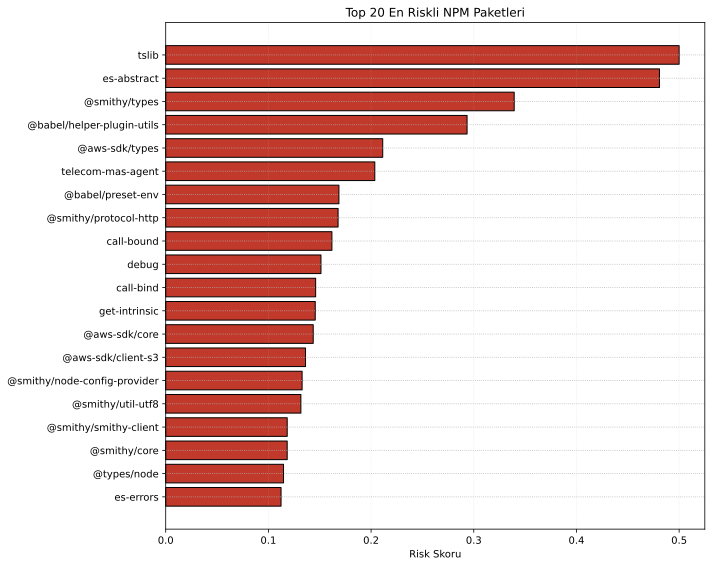
\includegraphics[width=\linewidth]{top20_risk_scores.png}
\caption{Top 20 packages by Composite Risk Score (BRS).}
\label{fig:risk_scores}
\end{figure}

\begin{table}[H]
\centering
\caption{\textsc{Top 20 Packages by Composite Risk Score (BRS)}}
\label{tab:risk}
\resizebox{\linewidth}{!}{%
\begin{tabular}{lrrrrr}
\toprule
Package & Risk & In-Degree & Out-Degree & Betweenness & TopN? \\
\midrule
@babel/helper-plugin-utils & 0.500000 & 110 & 0 & 0.000000 & True \\
@babel/core & 0.388827 & 12 & 15 & 0.001112 & True \\
jest-circus & 0.361688 & 1 & 20 & 0.001144 & False \\
jest-runner & 0.334157 & 2 & 22 & 0.001000 & True \\
get-intrinsic & 0.330606 & 22 & 10 & 0.000771 & True \\
babel-jest & 0.313975 & 2 & 7 & 0.001087 & True \\
@babel/helper-create-class-features-plugin & 0.274757 & 10 & 7 & 0.000798 & True \\
call-bound & 0.266206 & 41 & 2 & 0.000283 & False \\
@babel/traverse & 0.248118 & 20 & 7 & 0.000523 & True \\
es-abstract & 0.231558 & 17 & 54 & 0.000000 & False \\
jest-snapshot & 0.231168 & 6 & 21 & 0.000549 & True \\
@babel/preset-env & 0.213636 & 3 & 70 & 0.000000 & True \\
@babel/types & 0.212942 & 32 & 2 & 0.000236 & True \\
postcss-preset-env & 0.195974 & 1 & 67 & 0.000000 & True \\
@jest/types & 0.193414 & 26 & 7 & 0.000211 & True \\
debug & 0.183565 & 34 & 1 & 0.000100 & True \\
babel-preset-current-node-syntax & 0.182762 & 2 & 15 & 0.000499 & False \\
postcss-value-parser & 0.177273 & 39 & 0 & 0.000000 & True \\
call-bind & 0.175065 & 36 & 4 & 0.000000 & False \\
@types/node & 0.174844 & 34 & 1 & 0.000067 & False \\
\bottomrule
\end{tabular}%
}
\end{table}

\subsection{Systemic Impact and Cascade Analysis}
The simulation results support the validity of the BRS model. As shown in Figure \ref{fig:impact}, the removal of high-BRS packages causes a significant decrease in the LCC size. The correlation between the BRS score and the resulting cascade effect (Figure \ref{fig:cascade}) demonstrates the utility of the metric for risk prediction.

\begin{figure}[H]
\centering
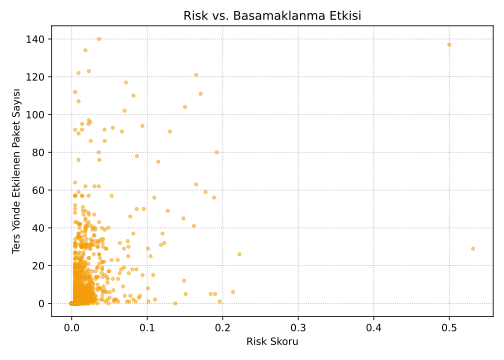
\includegraphics[width=\linewidth]{risk_vs_cascade.png}
\caption{Relationship between BRS and cascade effect, measured by network accessibility.}
\label{fig:cascade}
\end{figure}

\begin{figure}[H]
\centering
\includegraphics[width=\linewidth]{top20_cascade_impact.png}
\caption{Effect of removing the top 20 high-BRS packages on LCC size and network accessibility.}
\label{fig:impact}
\end{figure}

\section{Discussion}
This study presented the Composite Risk Score (BRS), a model that transforms the structural risks in the npm ecosystem into a measurable value, moving beyond the descriptive analyses common in the literature. The BRS ranking addresses the need for operational prioritization outlined in the Introduction. The analysis shows that network security depends not only on popular packages but also on infrastructural "bridge" packages such as \texttt{jest-circus} and \texttt{@babel/core}. These findings confirm the "small-world" network structure identified by Zimmermann et al. \cite{zimmermann2019smallworld}, but extend the literature by showing that risk is concentrated not only in popular packages but also in intermediate-layer packages that function as bridges.

The "Cascade Impact" simulations were performed on the constructed dependency graph rather than the entire npm registry, due to computational complexity. This approach relies on the "supply chain backbone" hypothesis, wherein the topological disintegration (loss of the LCC) of this dense network of critical packages serves as a mathematical proxy for the functional failure of dependent projects. Therefore, the structural collapse of this local backbone is interpreted as a direct indicator of global systemic risk.

\section{Limitations}
This analysis is limited to the static dependencies defined in \texttt{package.json} files. Packages loaded dynamically at runtime and the reputation of developer accounts were excluded. The analysis was also performed on a static snapshot of the ecosystem and does not include its temporal evolution. Finally, legal risks such as license compliance are outside the scope of this study \cite{ahlstrom2025licensing}.

\section{Conclusion}
This study proposed a topology-based methodology for identifying and prioritizing structurally critical packages in the npm software supply chain. By synthesizing multiple network metrics into a Behavioral Risk Score (BRS), we provide a quantitative framework to guide security resource allocation. The findings indicate that focusing on a small number of structurally critical nodes is a more efficient strategy for mitigating systemic risk than focusing on popularity alone. Future work should expand the model to include developer social networks and package maintenance behaviors, and apply the methodology to other package ecosystems to develop more generalized supply chain security models.

\section{Reproducibility}
The source code and datasets used in this study are available to ensure reproducibility.
\begin{itemize}
  \item \textbf{Analysis Code:} The analysis is contained in \texttt{analysis/analysis.ipynb} (Python 3, NetworkX, pandas).
  \item \textbf{Data Outputs:} All intermediate results and metrics are available in CSV format in the \texttt{results/} directory.
\end{itemize}

% APA-style bibliography 
\begin{thebibliography}{30}

\bibitem{lit1} E. Wyss, ``A new frontier for software security: Diving deep into npm,'' 2025.

\bibitem{lit7} M. Wang, P. Wu, and Q. Luo, ``Construction of software supply chain threat portrait based on chain perspective,'' 2023.

\bibitem{lit8} C. Liu et al., ``Demystifying vulnerability propagation via dependency trees in npm,'' in \textit{ICSE}, 2022.

\bibitem{lit18} A. Zerouali et al., ``On the impact of security vulnerabilities in the npm and RubyGems dependency networks,'' 2022.

\bibitem{lit5} I. Rahman et al., ``Characterizing dependency update practice of NPM, PyPI and Cargo packages,'' 2024.

\bibitem{lit22} F. R. Cogo, ``Studying dependency maintenance practices through mining NPM,'' 2020.

\bibitem{lit10} A. J. Jafari et al., ``Dependency practices for vulnerability mitigation,'' 2023.

\bibitem{lit20} M. Zimmermann et al., ``Small world with high risks: Security threats in npm,'' in \textit{USENIX Sec.}, 2019.

\bibitem{lit16} A. Hafner, A. Mur, and J. Bernard, ``Node package manager's dependency network robustness,'' 2021.

\bibitem{lit25} E.-R. Oldnall, ``The web of dependencies: A complex network analysis of the NPM,'' 2017.

\bibitem{lit2} P. Jaisri, B. Reid, and R. G. Kula, ``A preliminary study on self-contained libraries in the NPM ecosystem,'' 2024.

\bibitem{lit6} T. G. Hastings, ``Combating source poisoning and next-generation software supply chain attacks,'' 2024.

\bibitem{lit30} M. Shcherbakov, P. Moosbrugger, and M. Balliu, ``Unveiling the invisible: Prototype pollution gadgets via dynamic taint,'' 2021.

\bibitem{lit12} D. Y. K. Yip, ``Empirical study on dependency-based attacks in Node.js,'' 2022.

\bibitem{lit4} M. Ohm et al., ``Backstabber's knife collection: A review of open source software supply chain attacks,'' in \textit{DIMVA}, 2020.

\bibitem{lit24} P. Ladisa et al., ``The hitchhiker's guide to malicious third-party dependencies,'' in \textit{IEEE S\&P}, 2023.

\bibitem{lit28} R. Duan et al., ``Towards measuring supply chain attacks on package managers,'' in \textit{NDSS}, 2020.

\bibitem{lit19} A. Sejfia and M. Schafer, ``Practical automated detection of malicious npm packages (Amalfi),'' in \textit{ICSE}, 2022.

\bibitem{lit29} X. Zheng et al., ``Towards robust detection of OSS supply chain poisoning (OSCAR),'' 2024.

\bibitem{lit15} S. Halder et al., ``Malicious package detection using metadata information,'' 2024.

\bibitem{lit14} J. Zhang et al., ``Malicious package detection in NPM and PyPI using a single model of malicious behavior sequence,'' 2023.

\bibitem{lit17} P. Ladisa et al., ``On the feasibility of cross-language detection of malicious packages in npm and PyPI,'' 2023.

\bibitem{lit11} M. L. P. Correia, ``Detection of software supply chain attacks in code repositories,'' 2022.

\bibitem{lit23} M. Ohm et al., ``Supporting detection via unsupervised signature generation (ACME),'' 2021.

\bibitem{lit13} S. Torres-Arias, ``In-toto: Practical software supply chain security,'' in \textit{USENIX Sec.}, 2020.

\bibitem{lit3} S. Yu, ``Accurate and efficient SBOM generation for software supply chain security,'' 2024.

\bibitem{lit9} H. E. Ahlstrom, ``Dependency analysis for software licensing and security,'' 2025.

\bibitem{lit21} T. R. Schorlemmer, ``Software supply chain security: Attacks, defenses, and signing adoption,'' 2024.

\bibitem{lit26} N. Imtiaz, ``Toward secure use of open source dependencies,'' 2023.

\bibitem{lit27} S. Vaidya, ``Towards ensuring integrity and authenticity of software repositories,'' 2022.

\end{thebibliography}


\end{document}
